%% ============================================================================
%% fig_2_2_preprocessing_flow.tex -- TikZ source of thesis Figure 8 (label
%% fig:preprocessing_flow). Every label was checked
%% against the UNI extraction notebook (01-data-preparation, cells 4 and 6), the
%% v20 training notebook (feature formats), the CLAM patching defaults, the
%% recorded bag sizes and the preprocessing text of Chapter 2:
%%   - UNI (extracted for the thesis): HSV-saturation tissue mask on a
%%     low-resolution level (CLAM defaults 8 / 7 / 4); non-overlapping 256 px
%%     patches at 20x read at level 0; kept if >= 50% tissue; low-saturation and
%%     dark patches dropped; resized to 224 px; frozen UNI ViT-L/16 -> 1,024-d;
%%     .pt per slide with features N x 1024 and level-0 coordinates N x 2.
%%   - UNI2-h: features pre-extracted and released by MahmoodLab (CLAM-based
%%     patching, 256 px at 20x, level 0); .h5 per slide, N x 1536 + coordinates.
%%   - bag sizes as worded in Chapter 2; 24 configurations on the same five
%%     slide-level folds; no aggregator internals (Fig. 7 covers them).
%% Sizes (KTU thesis guide, section 5.1: figure text >= 10 pt): every text item 10.1 pt
%% (math sub/superscripts at the standard 7 pt script size of 10 pt text); stage
%% column, lanes and rows proportioned for that size (tall rows, wide lanes).
%% Natural width ~15.45 cm: include at \includegraphics[width=\textwidth] (scale ~1).
%% ============================================================================
\documentclass[border=1pt]{standalone}
\usepackage{newtxtext,newtxmath}
\usepackage{amsmath}
\usepackage{tikz}
\usetikzlibrary{arrows.meta}

% ---- sizes: printed >= 10 pt at scale ~1 (10.1 TeX pt = 10.06 bp) ----
\newcommand{\bodysize}{\fontsize{10.1}{12.4}\selectfont}
\DeclareMathSizes{10.1}{10.1}{7.07}{5.05}

\begin{document}
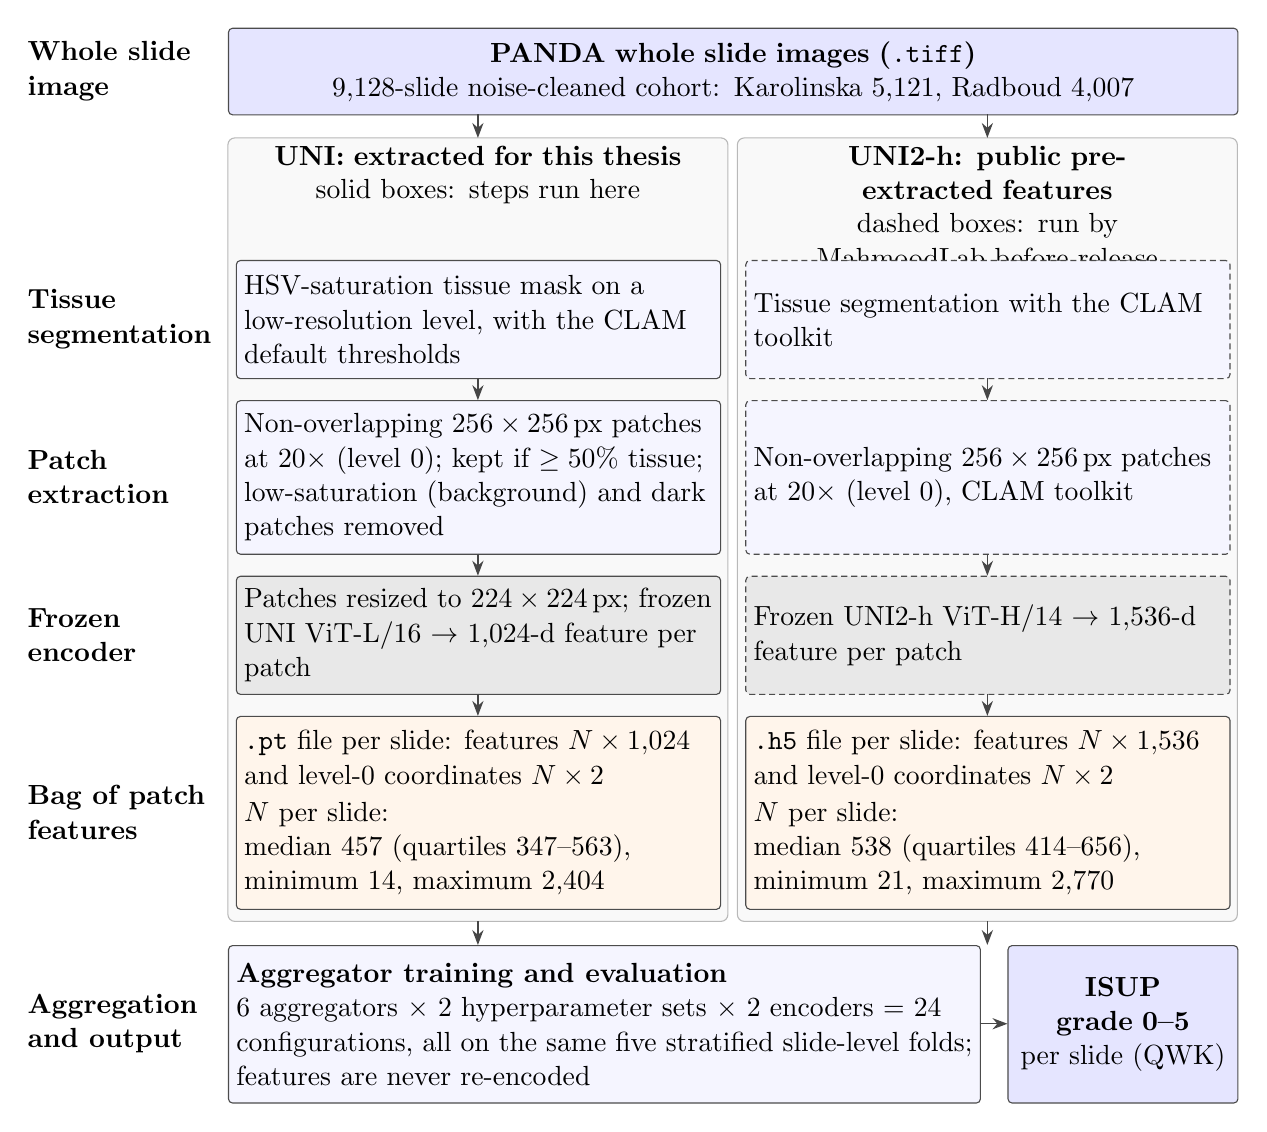
\begin{tikzpicture}[
  font=\bodysize,
  >={Stealth[length=1.9mm]},
  base/.style={draw=black!70, line width=0.4pt, rounded corners=1.5pt, anchor=north west,
               align=flush left, inner sep=0.1cm, execute at begin node={\hyphenpenalty=10000}},
  io/.style={base, fill=blue!10},
  proc/.style={base, fill=blue!4},
  frozen/.style={base, fill=gray!18},
  file/.style={base, fill=orange!8},
  prov/.style={dash pattern=on 2.2pt off 1.4pt},
  band/.style={draw=gray!55, line width=0.4pt, rounded corners=2.5pt, fill=gray!5},
  lab/.style={anchor=west, align=left, font=\bodysize\bfseries, inner sep=0pt},
  ttl/.style={anchor=north, align=center, inner sep=0pt, execute at begin node={\hyphenpenalty=10000}},
  ar/.style={->, line width=0.45pt, draw=gray!55!black}
]
% ---------------------------------------------------------------- geometry (cm)
% stage labels [0, 2.45]; lanes: UNI [2.55, 8.90], centre 5.725; UNI2-h [9.02, 15.37], centre 12.195
% boxes in a lane: x = lane + 0.10, text width 5.95 cm (box 6.15 cm)
% rows (top-bottom): R1 0.00-1.10 | band 1.40-11.35 (titles 1.50-2.80) |
%   R2 2.95-4.45 | R3 4.73-6.68 | R4 6.96-8.46 | R5 8.74-11.19 | R6 11.65-13.65

% ---------------------------------------------------------------- lane bands
\draw[band] (2.55,-1.40) rectangle (8.90,-11.35);
\draw[band] (9.02,-1.40) rectangle (15.37,-11.35);
\node[ttl, text width=6.15cm] at (5.725,-1.50)
  {\textbf{UNI: extracted for this thesis}\\[-0.5pt] solid boxes: steps run here};
\node[ttl, text width=6.15cm] at (12.195,-1.50)
  {\textbf{UNI2-h: public pre-extracted features}\\[-0.5pt] dashed boxes: run by MahmoodLab before release};

% ---------------------------------------------------------------- stage labels
\node[lab] at (0,-0.55)  {Whole slide\\image};
\node[lab] at (0,-3.70)  {Tissue\\segmentation};
\node[lab] at (0,-5.705) {Patch\\extraction};
\node[lab] at (0,-7.71)  {Frozen\\encoder};
\node[lab] at (0,-9.965) {Bag of patch\\features};
\node[lab] at (0,-12.65) {Aggregation\\and output};

% ---------------------------------------------------------------- R1 input (full width)
\node[io, text width=12.62cm, minimum height=1.10cm, align=center] (in) at (2.55,0)
  {\textbf{PANDA whole slide images (\texttt{.tiff})}\\
   9,128-slide noise-cleaned cohort: Karolinska 5,121, Radboud 4,007};

% ---------------------------------------------------------------- UNI lane
\node[proc, text width=5.95cm, minimum height=1.50cm] (u2) at (2.65,-2.95)
  {HSV-saturation tissue mask on a low-resolution level, with the CLAM default thresholds};
\node[proc, text width=5.95cm, minimum height=1.95cm] (u3) at (2.65,-4.73)
  {Non-overlapping $256\times256$\,px patches at $20\times$ (level~0); kept if $\geq 50\%$ tissue;
   low-saturation (background) and dark patches removed};
\node[frozen, text width=5.95cm, minimum height=1.50cm] (u4) at (2.65,-6.96)
  {Patches resized to $224\times224$\,px; frozen UNI ViT-L/16 $\rightarrow$ 1,024-d feature per patch};
\node[file, text width=5.95cm, minimum height=2.45cm] (u5) at (2.65,-8.74)
  {\texttt{.pt} file per slide: features $N\times1{,}024$ and \mbox{level-0} coordinates $N\times2$\\[1pt]
   $N$ per slide:\\ median 457 (quartiles \mbox{347--563}),\\ minimum 14, maximum 2,404};

% ---------------------------------------------------------------- UNI2-h lane
\node[proc, prov, text width=5.95cm, minimum height=1.50cm] (h2) at (9.12,-2.95)
  {Tissue segmentation with the CLAM toolkit};
\node[proc, prov, text width=5.95cm, minimum height=1.95cm] (h3) at (9.12,-4.73)
  {Non-overlapping $256\times256$\,px patches at $20\times$ (level~0), CLAM toolkit};
\node[frozen, prov, text width=5.95cm, minimum height=1.50cm] (h4) at (9.12,-6.96)
  {Frozen UNI2-h ViT-H/14 $\rightarrow$ 1,536-d feature per patch};
\node[file, text width=5.95cm, minimum height=2.45cm] (h5) at (9.12,-8.74)
  {\texttt{.h5} file per slide: features $N\times1{,}536$ and \mbox{level-0} coordinates $N\times2$\\[1pt]
   $N$ per slide:\\ median 538 (quartiles \mbox{414--656}),\\ minimum 21, maximum 2,770};

% ---------------------------------------------------------------- R6 aggregation and output
\node[proc, text width=9.35cm, minimum height=2.00cm] (agg) at (2.55,-11.65)
  {\textbf{Aggregator training and evaluation}\\
   6 aggregators $\times$ 2 hyperparameter sets $\times$ 2 encoders $=$ 24 configurations, all on the
   same five stratified slide-level folds; features are never re-encoded};
\node[io, text width=2.72cm, minimum height=2.00cm, align=center] (out) at (12.45,-11.65)
  {\textbf{ISUP grade 0--5}\\ per slide (QWK)};

% ---------------------------------------------------------------- arrows
\foreach \x in {5.725, 12.195} {
  \draw[ar] (\x,-1.10) -- (\x,-1.40);   % input -> lane
  \draw[ar] (\x,-4.45) -- (\x,-4.73);   % segmentation -> patches
  \draw[ar] (\x,-6.68) -- (\x,-6.96);   % patches -> encoder
  \draw[ar] (\x,-8.46) -- (\x,-8.74);   % encoder -> feature file
  \draw[ar] (\x,-11.35) -- (\x,-11.65); % lane -> aggregation
}
\draw[ar] (12.10,-12.65) -- (12.45,-12.65);
\end{tikzpicture}
\end{document}
